\newcounter{nuserstory}
\newcounter{nusecase}

\newcommand{\userstory}[4]{%
    \refstepcounter{nuserstory}
    \subsection{#1}
    \label{userstory:\thenuserstory}
    \hangindent=40pt
    \textbf{\textit{As a}} #2,\\
    \textbf{\textit{I want to}} #3,\\
    \textbf{\textit{so that}} #4.
}
\newenvironment{usecase}[1]
{
    \refstepcounter{nusecase}%
    \subsection{Use Case \thenusecase: #1}%
    \label{usecase:\thenusecase}%
}{}

% With user stories (\userstory) you can reference them back later with \ref{userstory:n}
% For example, first user story in this file can be referred with \ref{userstory:1}

\chapter{Requirement Analysis}
\label{chap:requirement-analysis}

\section{Stakeholder Analysis}
\label{section:stakeholder-analysis}

\subsection{Primary Stakeholders}
\label{subsection:primary-stakeholders}

\begin{enumerate}[leftmargin=80pt]
    \item \textbf{Users:} The primary stakeholders are the users of our multi-camera tracking system, including security personnel, facility managers, emergency response coordinators, and research analysts.  Their interaction with the system is crucial for effective monitoring, incident response, and data-driven decision-making.  For a detailed specification of our users, see \ref{section:target-user}.
    \item \textbf{System Administrators:}  These individuals are responsible for the installation, configuration, and maintenance of the system.  Their needs include ease of deployment, system stability, and access to diagnostic tools.
    \item \textbf{University/Factory Management:}  These stakeholders are interested in the overall benefits of the system, such as improved safety, optimized resource allocation, and enhanced operational efficiency.  They require reports and data summaries to justify the investment and track performance.
\end{enumerate}

\section{User Stories}
\label{section:user-stories}

%% User Stories Start

\userstory{Continuously Track Individuals Across the Area%
}{security officer%
}{continuously track individuals as they move throughout the monitored area, even when they move between different camera views%
}{I can maintain uninterrupted surveillance of persons of interest and respond quickly to developing situations.}

\userstory{Maintain Tracking During Brief Disappearances%
}{security officer%
}{maintain the track of individuals even if they are temporarily out of sight of all cameras%
}{I can have a complete picture of a person's movements, even if they briefly go around corners or into areas without direct camera coverage.}

\userstory{Visualize Movement Paths%
}{facility manager%
}{see a visual representation of how people move through the facility, including their paths and locations over time%
}{I can understand space usage, identify congestion points, and make informed decisions about facility layout and resource allocation.}

\userstory{Access Historical Movement Data%
}{analytics specialist%
}{access and analyze historical data on individual and group movements, including options to export this data%
}{I can perform in-depth analysis of movement patterns, identify trends, and generate reports to improve operational efficiency and space utilization.  I can also share this data with other systems.}

\userstory{Prioritize Tracking of Specific Individuals%
}{security officer/emergency coordinator%
}{designate specific individuals for increased monitoring and receive immediate updates on their location%
}{I can focus on persons of interest during security incidents or emergencies, ensuring a rapid and effective response.}

\userstory{Ensure System Reliability and Uptime%
}{system administrator%
}{easily monitor system performance, troubleshoot issues, and perform necessary maintenance tasks%
}{I can keep the tracking system running smoothly and minimize disruptions to users.}
%% User Stories End

\section{Use Case Diagram}
\label{section:use-case-diagram}

% \begin{figure}[h!]
%     \centering
%     \begin{tikzpicture}

%         \begin{umlsystem}[x=4]{KU Eater}
%             \umlusecase[name=signup, y=4.5]{Sign Up}
%             \umlusecase[name=login, y=3]{Login}
%             \umlusecase[name=viewrec, y=1, width=2.5cm]{View Recommendations}
%             \umlusecase[name=genrec, x=6.5, y=2, width=2.5cm]{Generate Recommendations}
%             \umlusecase[name=menuinfo, x=4, y=0.25]{See Menu Info}
%             \umlusecase[name=searchmenu, x=1, y=-1]{Search Menu Items}
%             \umlusecase[name=userrec, x=6.5, y=-4, width=3.5cm]{Personalized Recommendations}
%             \umlusecase[name=trendrec, x=6.5, y=4.5, width=2.5cm]{Trending Recommendations}
%             \umlusecase[name=readreview, y=-2.5]{Read Reviews}
%             \umlusecase[name=writereview, x=-0.25, y=-4]{Write Review}
%             \umlusecase[name=rateitem, x=1, y=-5.5]{Rate Menu Items}
%             \umlusecase[name=editprofile, x=3, y=-7]{Edit Profile}
%         \end{umlsystem}

%         \umlactor[y=-1]{User}
%         \umlactor[y=3]{Guest}
%         \umlactor[y=-5]{Member}
%         \umlactor[x=15]{System}

%         \umlassoc{Guest}{login}
%         \umlassoc{Guest}{signup}
%         \umlassoc{User}{viewrec}
%         \umlassoc{User}{menuinfo}
%         \umlassoc{User}{searchmenu}
%         \umlassoc{User}{readreview}
%         \umlassoc{Member}{writereview}
%         \umlassoc{Member}{rateitem}
%         \umlassoc{Member}{editprofile}
%         \umlassoc{System}{genrec}
%         \umlinclude{viewrec}{genrec}
%         \umlinclude{userrec}{writereview}
%         \umlinclude{userrec}{rateitem}
%         \umlinclude{userrec}{editprofile}
%         \umlinherit{Guest}{User}
%         \umlinherit{Member}{User}
%         \umlinherit{userrec}{genrec}
%         \umlinherit{trendrec}{genrec}

%     \end{tikzpicture}
%     \caption{Use Case Diagram of KU Eater}
%     \label{fig:use-case-diagram}
%     \vspace*{-1in}
% \end{figure}

% Use case diagram (Figure \ref{fig:use-case-diagram}) is a visualization of functionalities that KU Eater provides for end-users. We decided to break
% down the users \textit{(on the left side of figure)} into three groups:

% \begin{itemize}
%     \item \textbf{\textit{User}}---a default group of users which has all the basic functionalities including: Viewing Recommendations, Seeing Menu Details,
%     Searching for Menu Items, and Reading Reviews.
%     \item \textbf{\textit{Guest}}---a group of user which extends from base functionalities, they are able to Sign Up and Login.
%     \item \textbf{\textit{Member}}---an authorized group of user, being able to Write Reviews, Rate Menu Items and Edit their Profiles.
% \end{itemize}
\section{Use Case Model}
\label{section:use-case-model}

\begin{usecase}{Track Individual Across Cameras}
    \textbf{Actors:} Security Officer
    
    \textbf{Description:} Track an individual's movements across multiple camera views.
    
    \textbf{Scenario:}
    \begin{enumerate}[leftmargin=80pt]
        \item Log into SpotOn.
        \item Select a location and date.
        \item View available camera feeds.
        \item See people with assigned IDs in each camera view.
        \item View a map showing detected individuals.
        \item Select an individual in any camera view.
        \item See that individual highlighted in all cameras where they appear.
        \item View their movement history on the map.
    \end{enumerate}
\end{usecase}

\begin{usecase}{Maintain Tracking During Temporary Disappearance}
    \textbf{Actors:} Security Officer
    
    \textbf{Description:} Continue tracking an individual even when temporarily out of camera view.
    
    \textbf{Scenario:}
    \begin{enumerate}[leftmargin=80pt]
        \item Track an individual in the system.
        \item When the person moves out of all camera views, the system marks this state.
        \item When the person reappears, the system reconnects their identity.
        \item See the individual's complete path, with estimated routes during gaps shown as dashed lines.
    \end{enumerate}
\end{usecase}

\begin{usecase}{Visualize Movement Paths on a Map}
    \textbf{Actors:} Facility Manager/Analytics Specialist
    
    \textbf{Description:} View movement patterns within a facility for space utilization analysis.
    
    \textbf{Scenario:}
    \begin{enumerate}[leftmargin=80pt]
        \item Log into SpotOn.
        \item Select a location and date.
        \item View a bird's-eye map of the facility.
        \item See movement paths of all individuals overlaid on the map.
        \item Filter paths by camera view.
        \item Select an individual to highlight only their path.
    \end{enumerate}
\end{usecase}

\begin{usecase}{Prioritize Tracking of Specific Individual}
    \textbf{Actors:} Security Officer/Emergency Coordinator
    
    \textbf{Description:} Focus system resources on tracking a specific individual.
    
    \textbf{Scenario:}
    \begin{enumerate}[leftmargin=80pt]
        \item Log into SpotOn.
        \item Select a location and date.
        \item View camera feeds and detected individuals.
        \item Designate an individual for prioritized tracking.
        \item See visual highlighting of the prioritized individual in all cameras.
        \item View their position, detection time, tracking duration, and movement details.
    \end{enumerate}
\end{usecase}

% Use Cases End
% \newpage

\section{User Interface Design}
\label{section:user-interface-design}

The user interface for the multi-camera tracking system is designed to offer a clear, intuitive, and efficient experience for security personnel, facility managers, and other stakeholders, focusing on retrospective analysis of recorded video feeds.  The interface prioritizes the visualization of movement patterns, easy access to detailed tracking information.
% Mockup Start

\begin{figure}[h!]
    \centering
    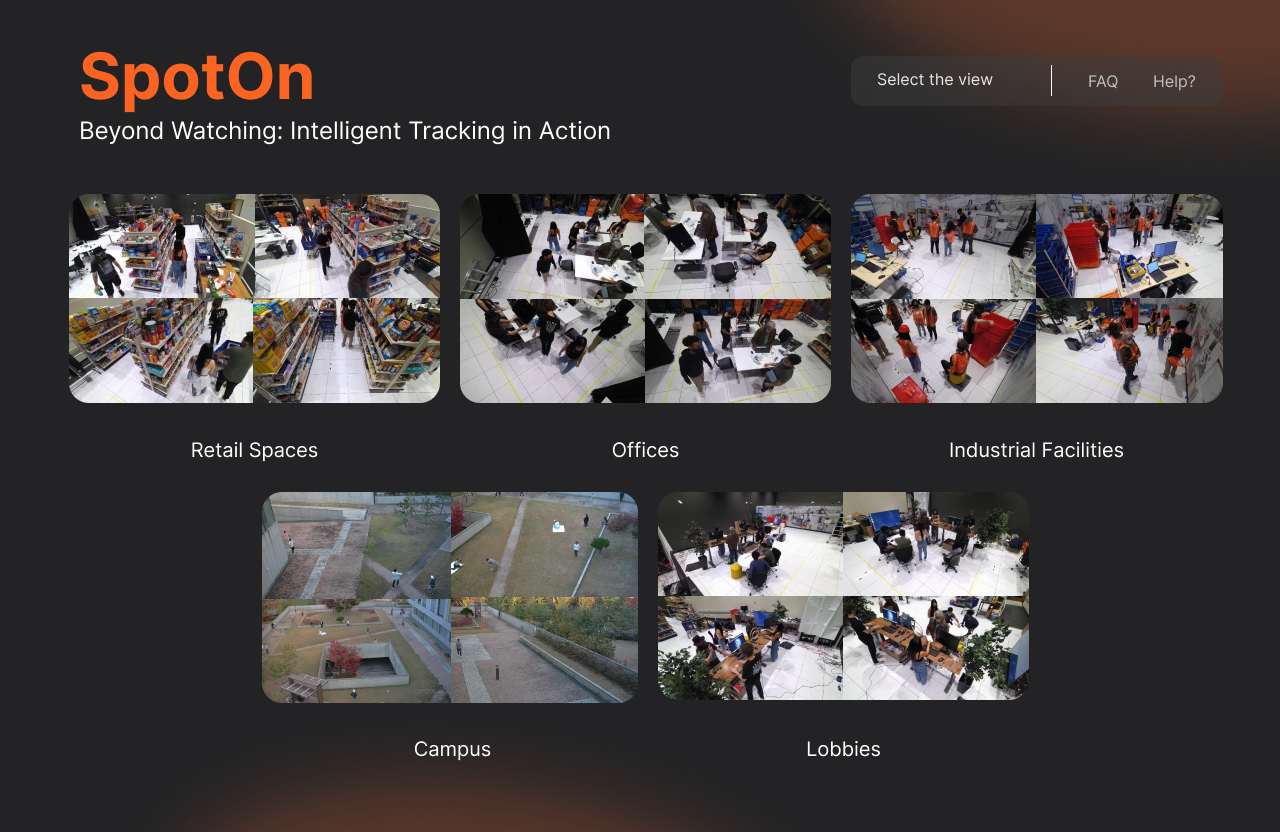
\includegraphics[width=0.8\textwidth,keepaspectratio]{jubjones/mockup/Dashboard.png}
    \caption{Mockup of Landing Page}
    \label{fig:mockup-landing-page}
\end{figure}

\begin{figure}[h!]
    \centering
    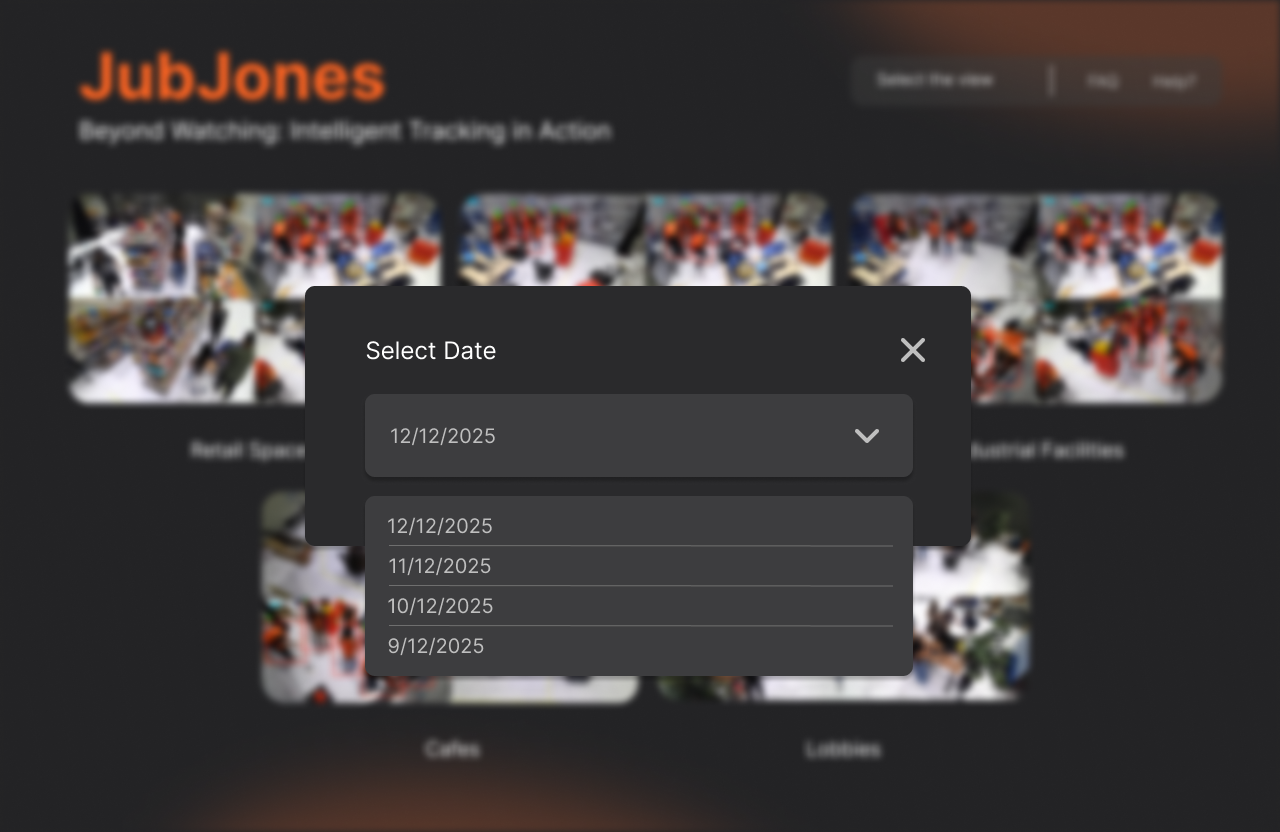
\includegraphics[width=0.8\textwidth,keepaspectratio]{jubjones/mockup/Dashboard - Select toggle.png}
    \caption{Mockup of Landing Page (Date Selection)}
        \label{fig:mockup-landing-page-datetime}
\end{figure}

\begin{figure}[h!]
    \centering
    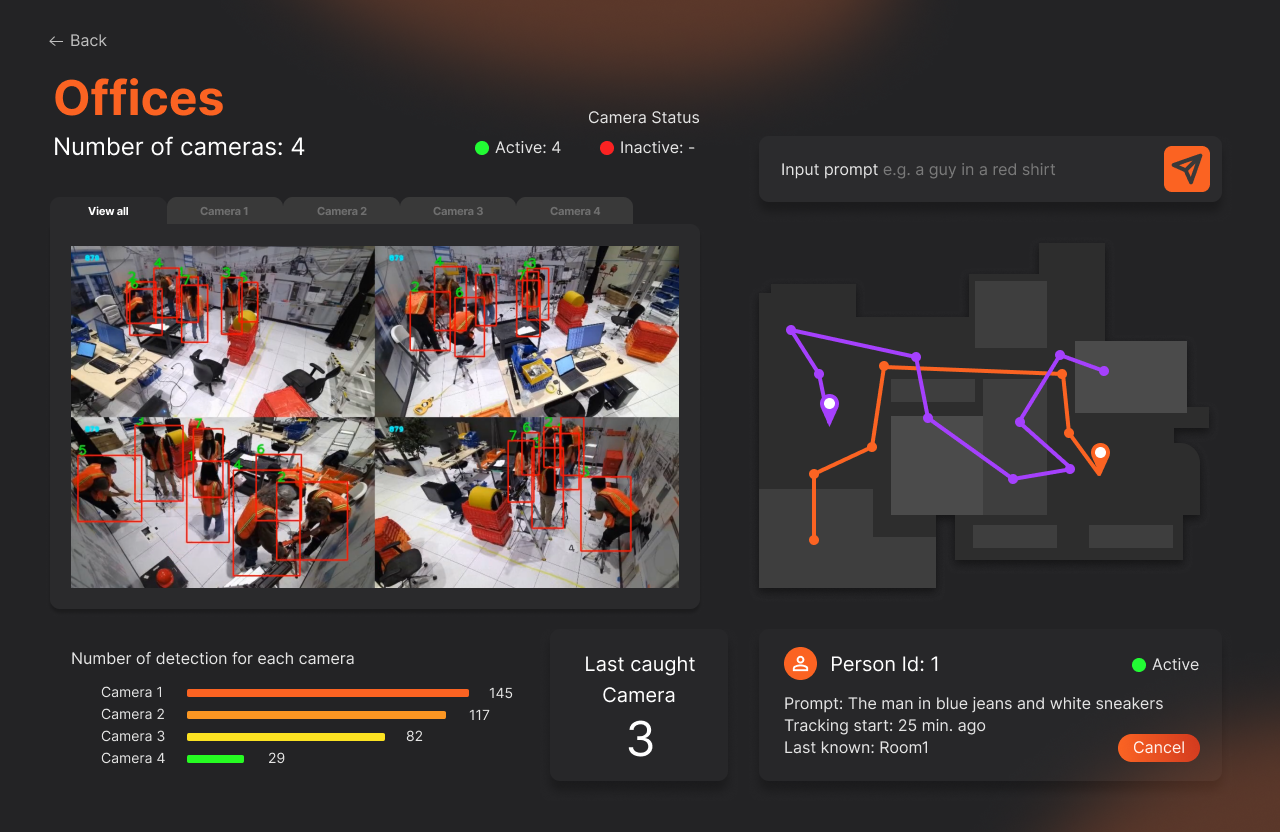
\includegraphics[width=0.8\textwidth,keepaspectratio]{jubjones/mockup/Group view.png}
    \caption{Mockup of Group View Page (Overview)}
    \label{fig:mockup-group-view}
\end{figure}

\begin{figure}[h!]
    \centering
    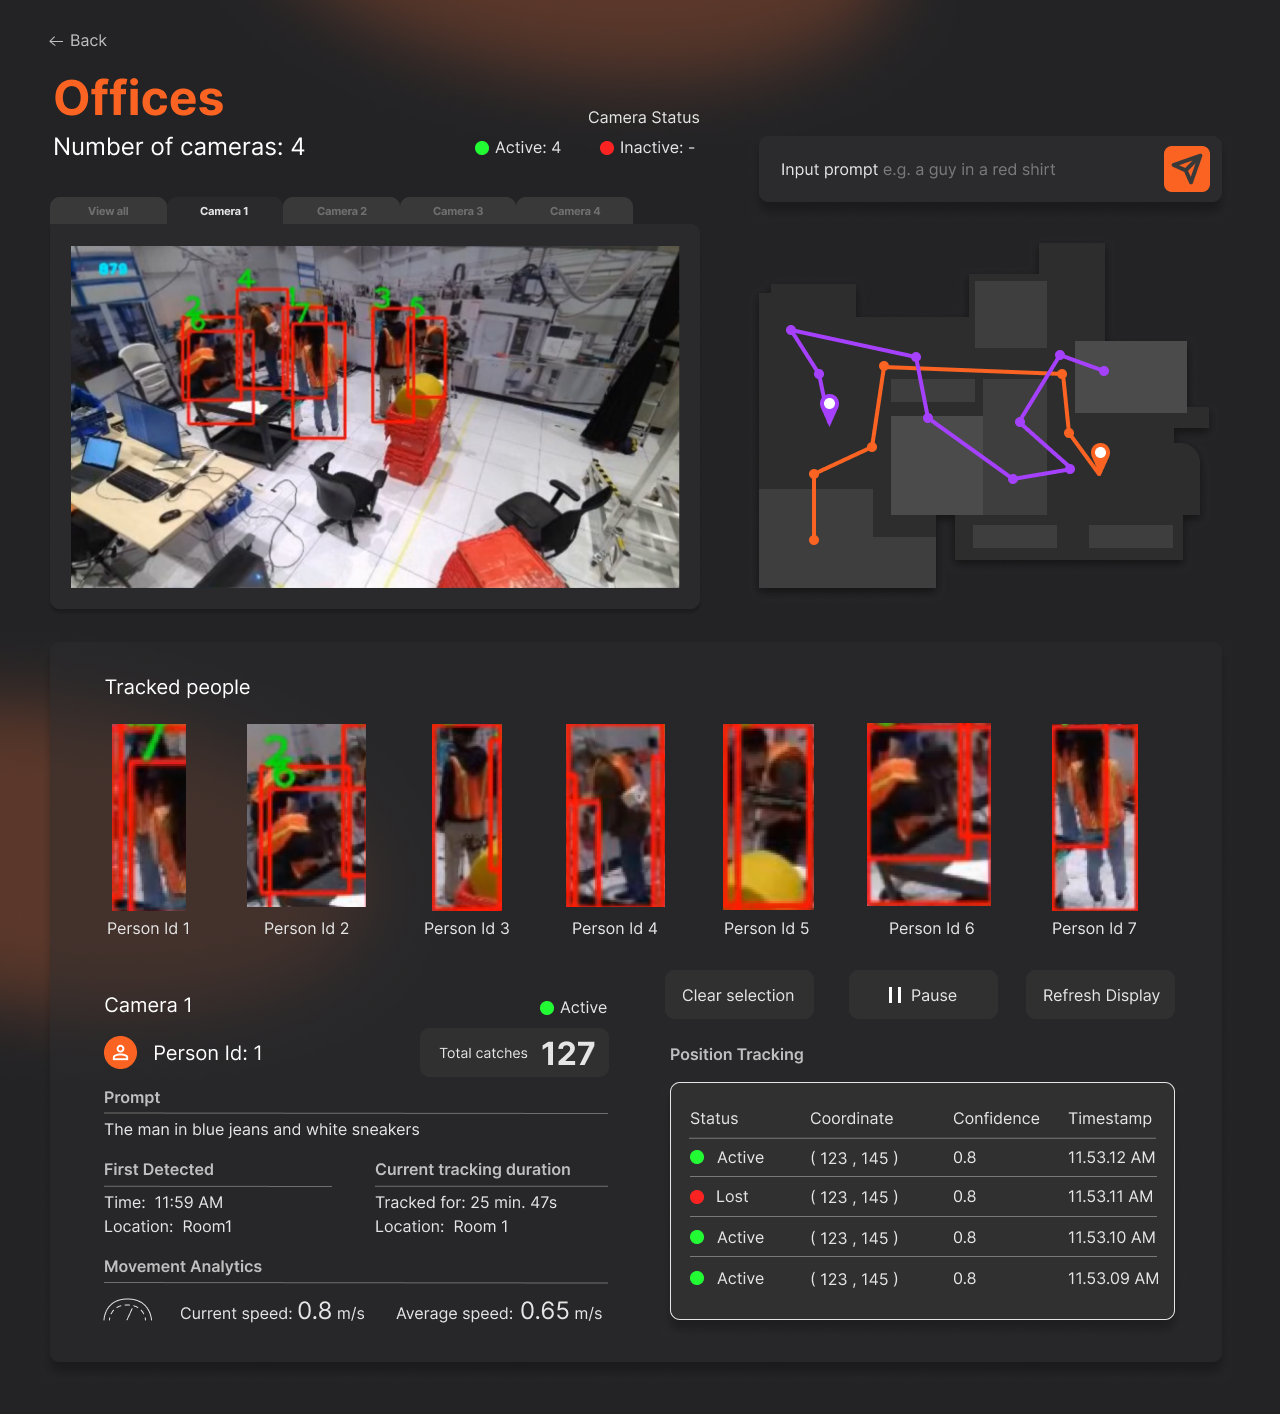
\includegraphics[width=0.8\textwidth, keepaspectratio]{jubjones/mockup/Detail view - expand.png} %Added height constraint
    \caption{Mockup of Group View Page (Expanded - Single Camera View)}
    \label{fig:mockup-group-view-expanded}
\end{figure}
\clearpage

% Mockup End
\newpage

\section{Target and Development System}
\label{section:development-system}

\subsection{Data Preparation}
\label{subsection:data-preparation-system}
% In order to prepare data for KU Eater, proper tooling is needed both for data storage and retrieval. The following list is the technologies we used in data preparation:

% \begin{itemize}[leftmargin=80pt]
%     \item \textbf{Google Sheets:} In order to record interview results such as stall information, list of menu items, we decided to use Google Sheets as our storage for raw data\footnote{The spreadsheet containing the data: \url{https://docs.google.com/spreadsheets/d/1oQ_PykNVvtV5KKtKOrva9aiZeK4S42EuFP9S6qaO4cg}}.
%     The advantage of this tool is that we have faster access to data, especially when we are doing interviews with data holders.
%     \item \textbf{PostgreSQL:} PostgreSQL is a relational database system, one of the advantages that PostgreSQL offers is the synchronous replication, we can use that feature in order to separate between the master data store, and sandbox database for training ML models.
%     PostgreSQL is used as our main datastore. PostgreSQL also has vector support for AI-driven applications.
% \end{itemize}

% \subsection{Recommendation Engine}
% \label{subsection:recommendation-engine}
% KU Eater at its core features a recommendation system, in order to build a consistent and fast service, we chose the following technologies:

% \begin{itemize}[leftmargin=80pt]
%     \item \textbf{gRPC:} A high performant protocol to do Remote Procedure Calls (RPC) that allows us to share schemas between
%     services. This allows for consistent data throughout the application's scope and predictable behavior.
%     \item \textbf{Tonic:} A gRPC server based on the Rust programming language. It is performant and can be
%     used to serve data asynchronously for a near real-time experience.
%     \item \textbf{PostgreSQL:} Like in the step of Data Preparation (\ref{subsection:data-preparation-system}), we can use replication to our advantage to update data in real-time
%     both from autonomous systems or administrator edits.
% \end{itemize}


% \subsection{Web Application}
% \label{subsection:web-application}
% KU Eater as a web-based mobile application, needs an interface designed with a target of mobile phone users in mind.
% In order to complement our requirements, our approach to the development process of the application must be mobile-first.
% The following is the technology stack of KU Eater web application:

% \begin{itemize}[leftmargin=80pt]
%     \item \textbf{React Native:} React Native is a framework based on React that offers powerful data fetching functionalities, built-in caching using existing web technologies etc. \\
%     The framework is native to Javascript, and can ensure its compatibility across devices. It is used as our frontend for the application and a mediator between the backend.
% \end{itemize}